\chapter{Implementation}
This section presents the implementation details of the full stack application developed during the project. It includes the methodology or proposal followed, the testing or verification plan, screenshots showcasing the output, and any relevant quality assurance measures taken.

\section{Methodology}
For the development of this project, a structured approach was adopted, which involved the following steps:

\begin{enumerate}
	\item \textbf{Requirement Gathering:} The initial phase involved gathering and analyzing the requirements for the full stack application. This included identifying the essential features, user interface design, and database structure.
	\begin{figure}[!h]
		\centering
		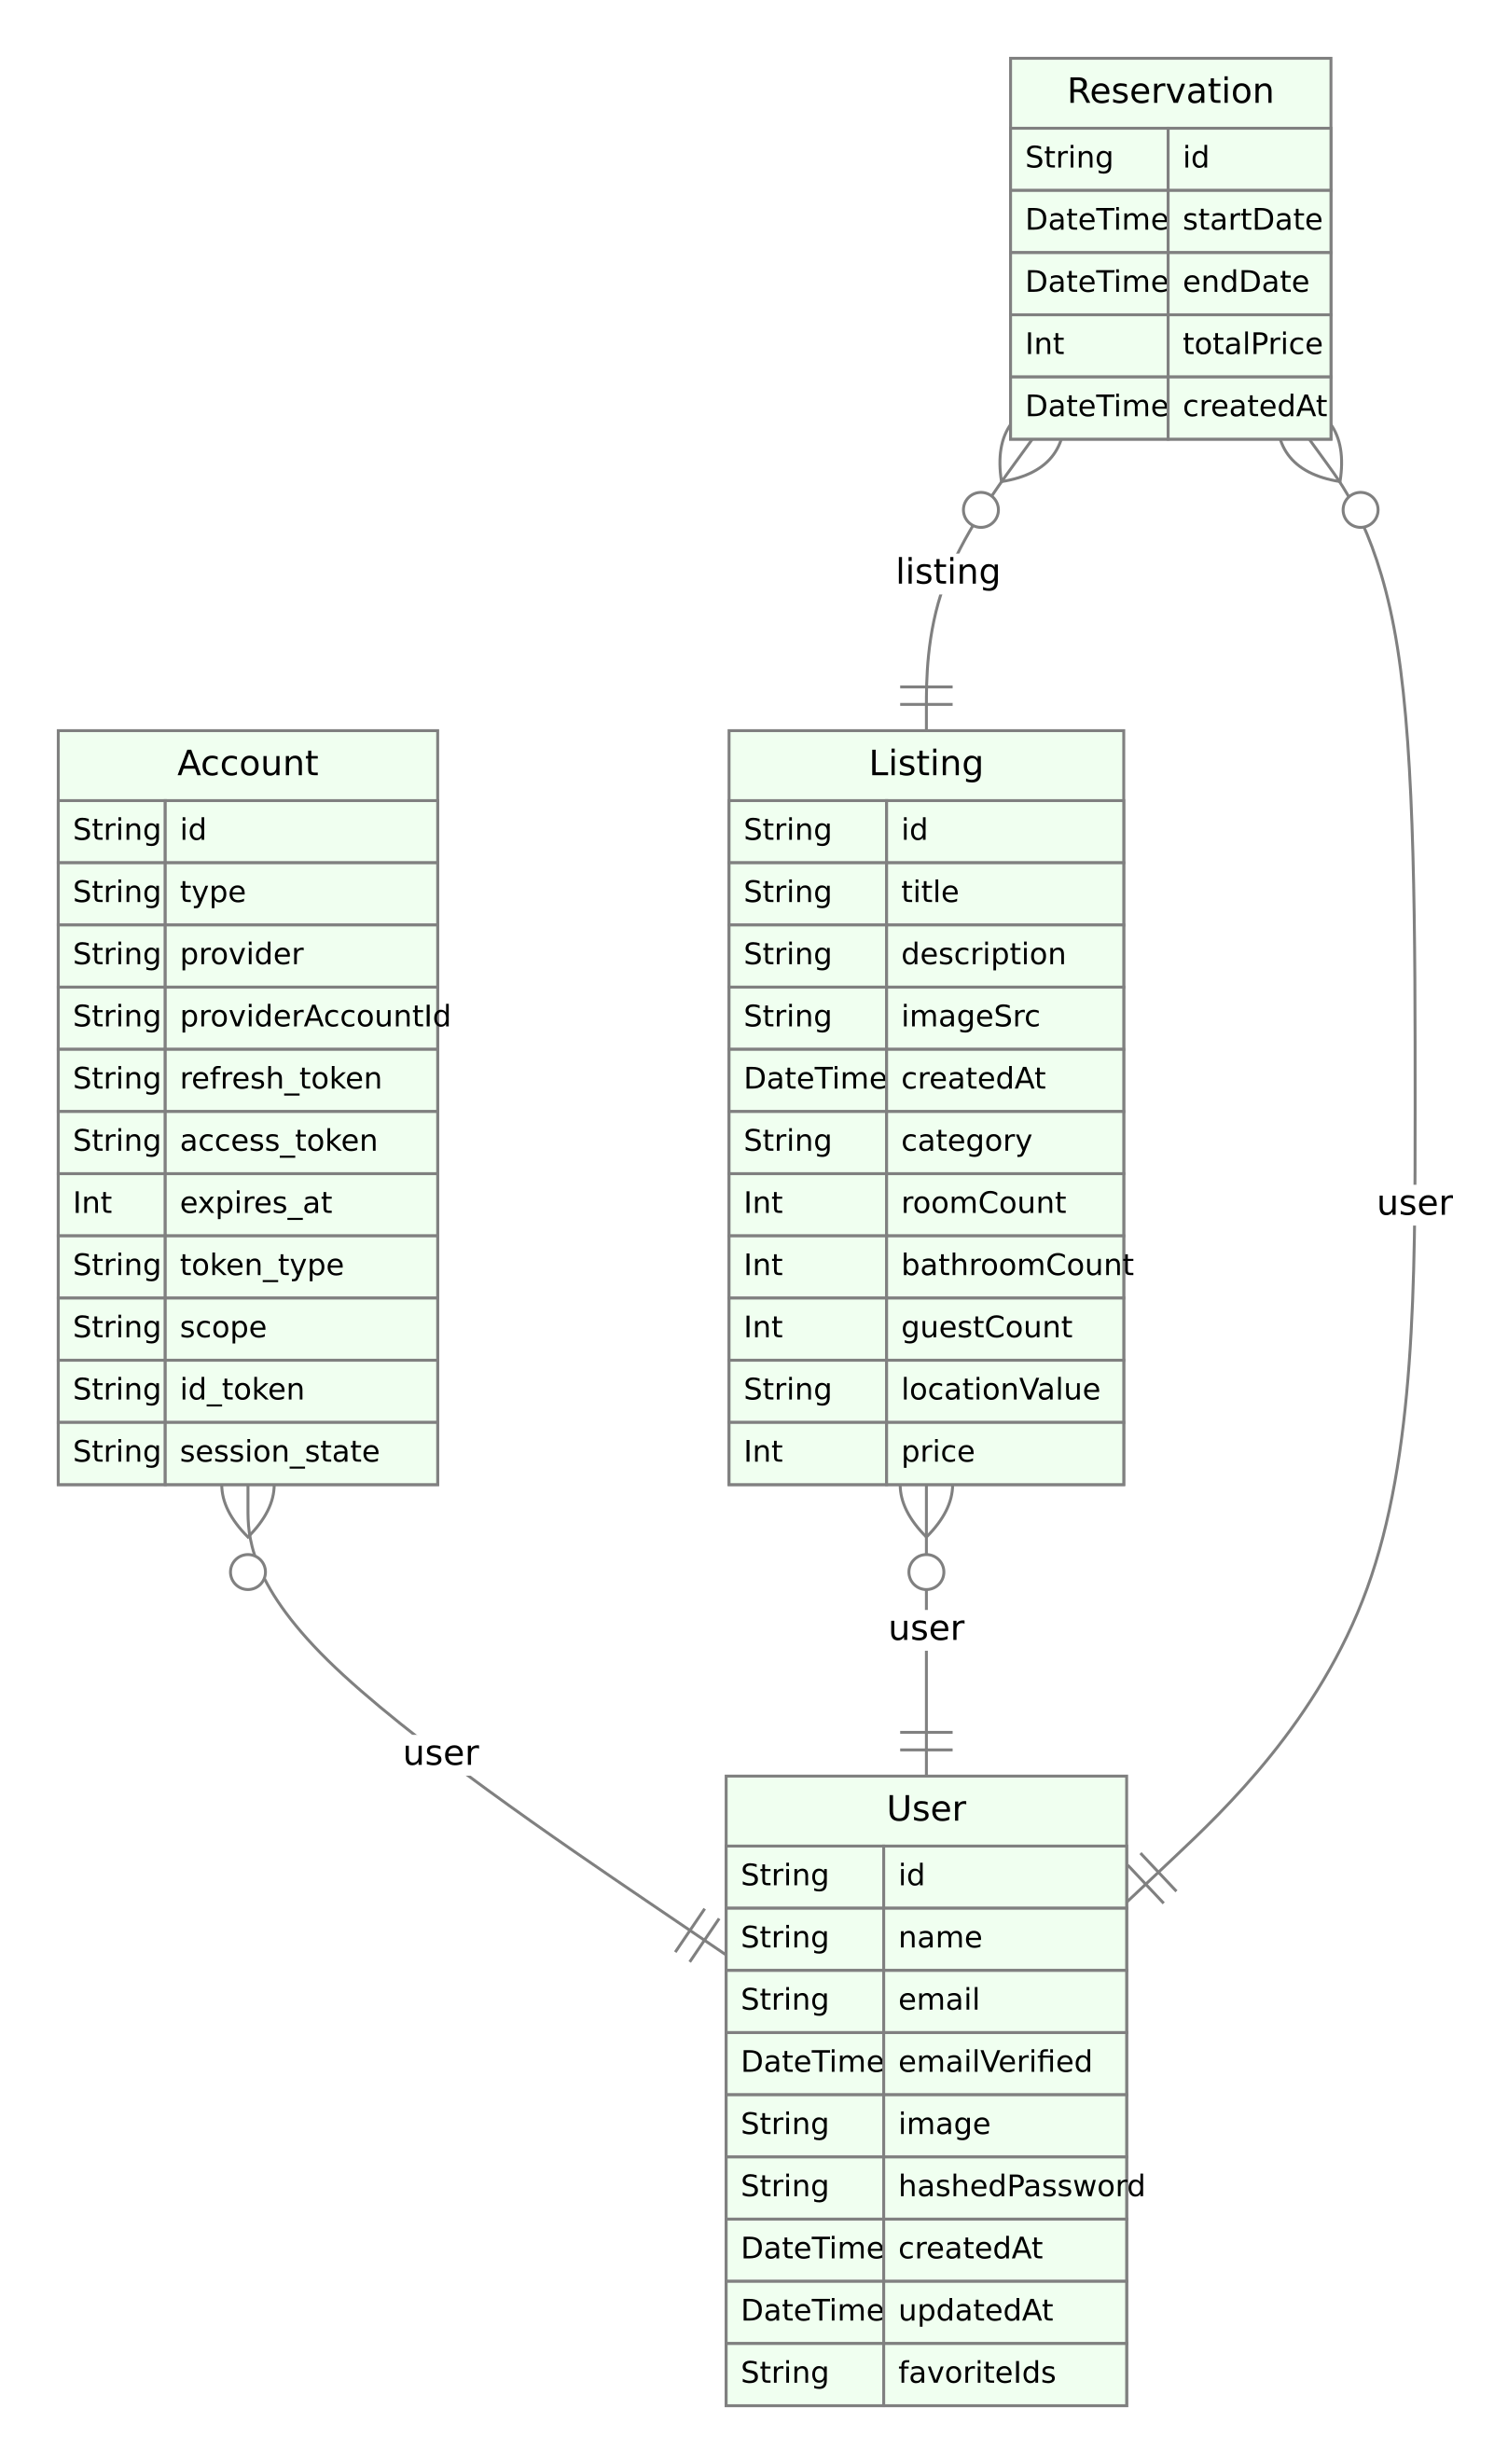
\includegraphics[scale=0.5]{chapters/images/erdiagram.png}
		\caption{ER Diagram}
	\end{figure}
	\item \textbf{System Design:} Based on the gathered requirements, a system design was formulated. This included the architectural design, database schema design, and UI/UX wireframing. The design phase focused on ensuring modularity, scalability, and a seamless user experience.
	\begin{figure}[!h]
		\centering
		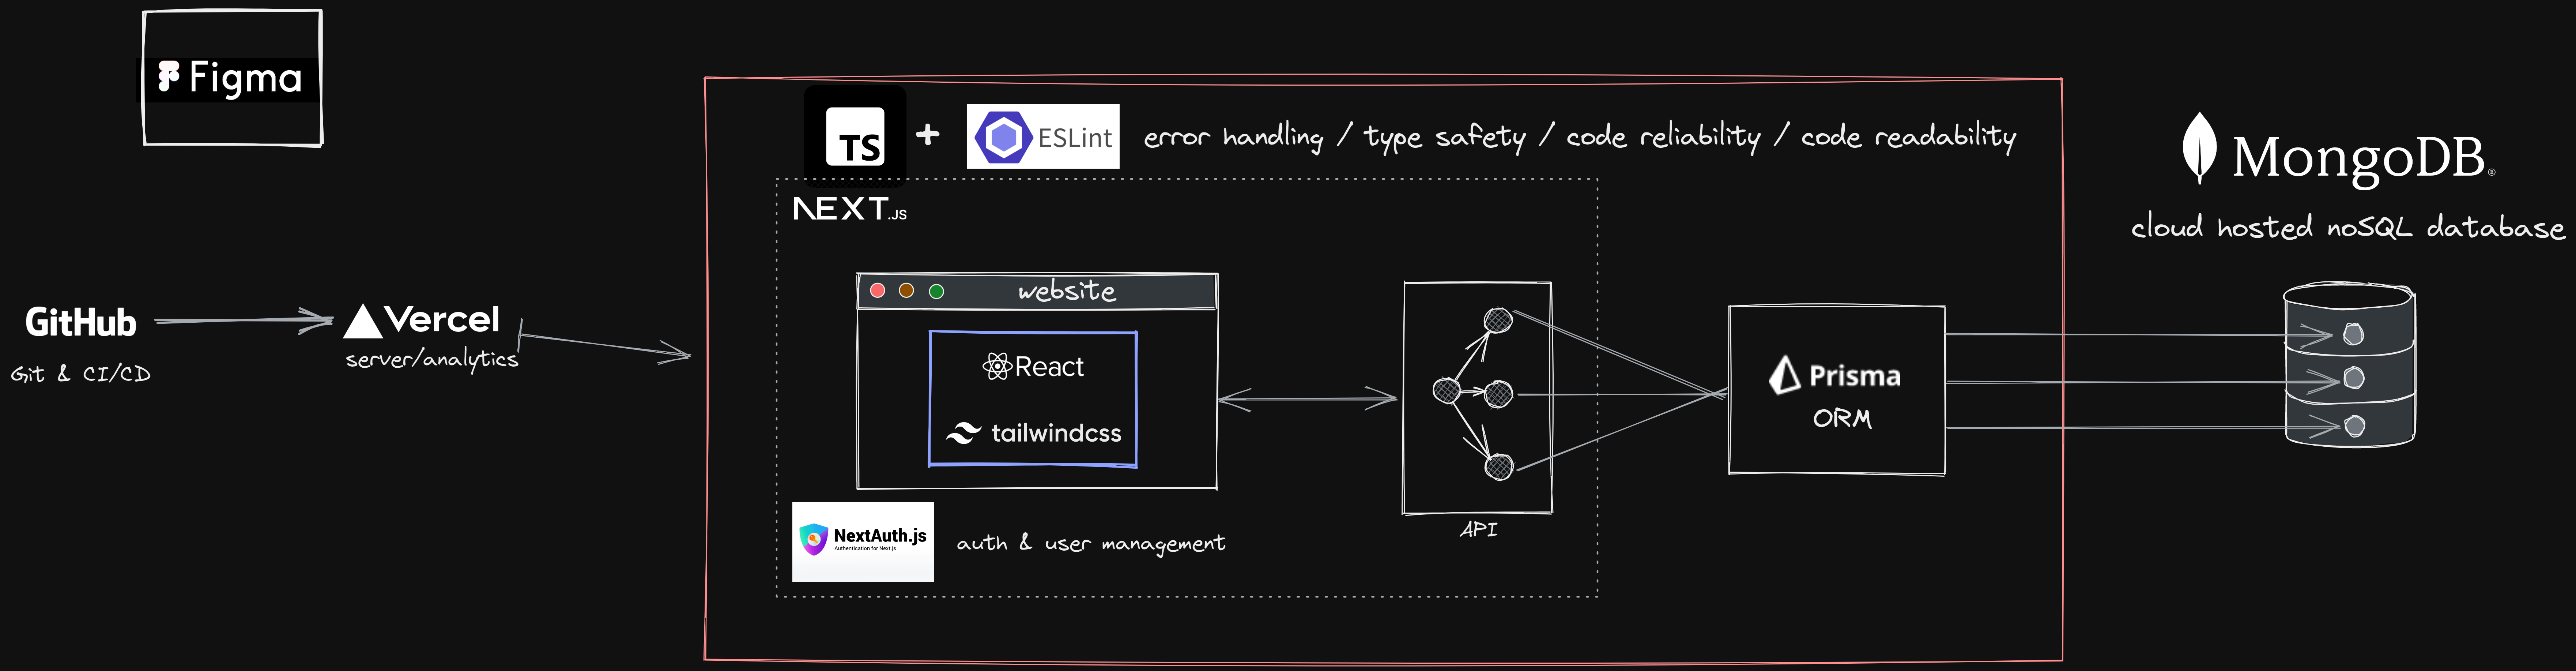
\includegraphics[scale=0.05]{chapters/images/airbnb-clone.png}
		\caption{System Architecture diagram}
	\end{figure}
	\item \textbf{Implementation:} The development phase involved coding the application using NextJS, Typescript, Prisma, TailwindCSS, MongoDB, and Cloudinary. Throughout the implementation, ESLint was integrated into the codebase to enforce coding standards and maintain consistency. ESLint rules and plugins were configured to check for errors, stylistic inconsistencies, and adherence to best practices.
	\item \textbf{Testing:} Although there was no dedicated QA team, testing was performed during the implementation phase. While unit testing and integration testing were not explicitly conducted, the application's functionality was manually tested to ensure its correctness and robustness.
	\item \textbf{Deployment:} Once the application was deemed stable and fully functional, it was deployed to a production environment. Continuous integration and continuous deployment (CI/CD) pipelines were set up to automate the deployment process, ensuring smooth and efficient updates.
\end{enumerate}

\section{Testing Plan}
Manual testing was performed to verify the outcome of the project. The testing plan included the following aspects:

\begin{enumerate}
	\item \textbf{Functionality Testing: } The application's features and functionalities were tested to ensure they worked as intended. This involved manually executing test cases that covered different user scenarios and workflows.
	\item \textbf{User Interface Testing: } The user interface was tested for responsiveness and visual consistency across different devices and screen sizes.
	\item \textbf{Usability Testing: } The application's usability and user experience were evaluated by soliciting feedback from users and incorporating their suggestions for improvements.
	\item \textbf{Error Handling Testing: } The application's error handling capabilities were tested by intentionally triggering various error scenarios and ensuring that appropriate error messages or fallbacks were displayed to the users.
	\item \textbf{Performace Testing: } The application's performance was evaluated by simulating high user loads and stress testing. This ensured that the application could handle a significant number of concurrent users without performance degradation.
\end{enumerate}

While unit testing and integration testing were not explicitly carried out, the manual testing approach aimed to identify and address any issues or bugs during the implementation phase.

\section{Screenshots}
The following screenshots provide a visual representation of the output and user interface of the implemented full stack application:

\begin{figure}[!h]
	\centering
	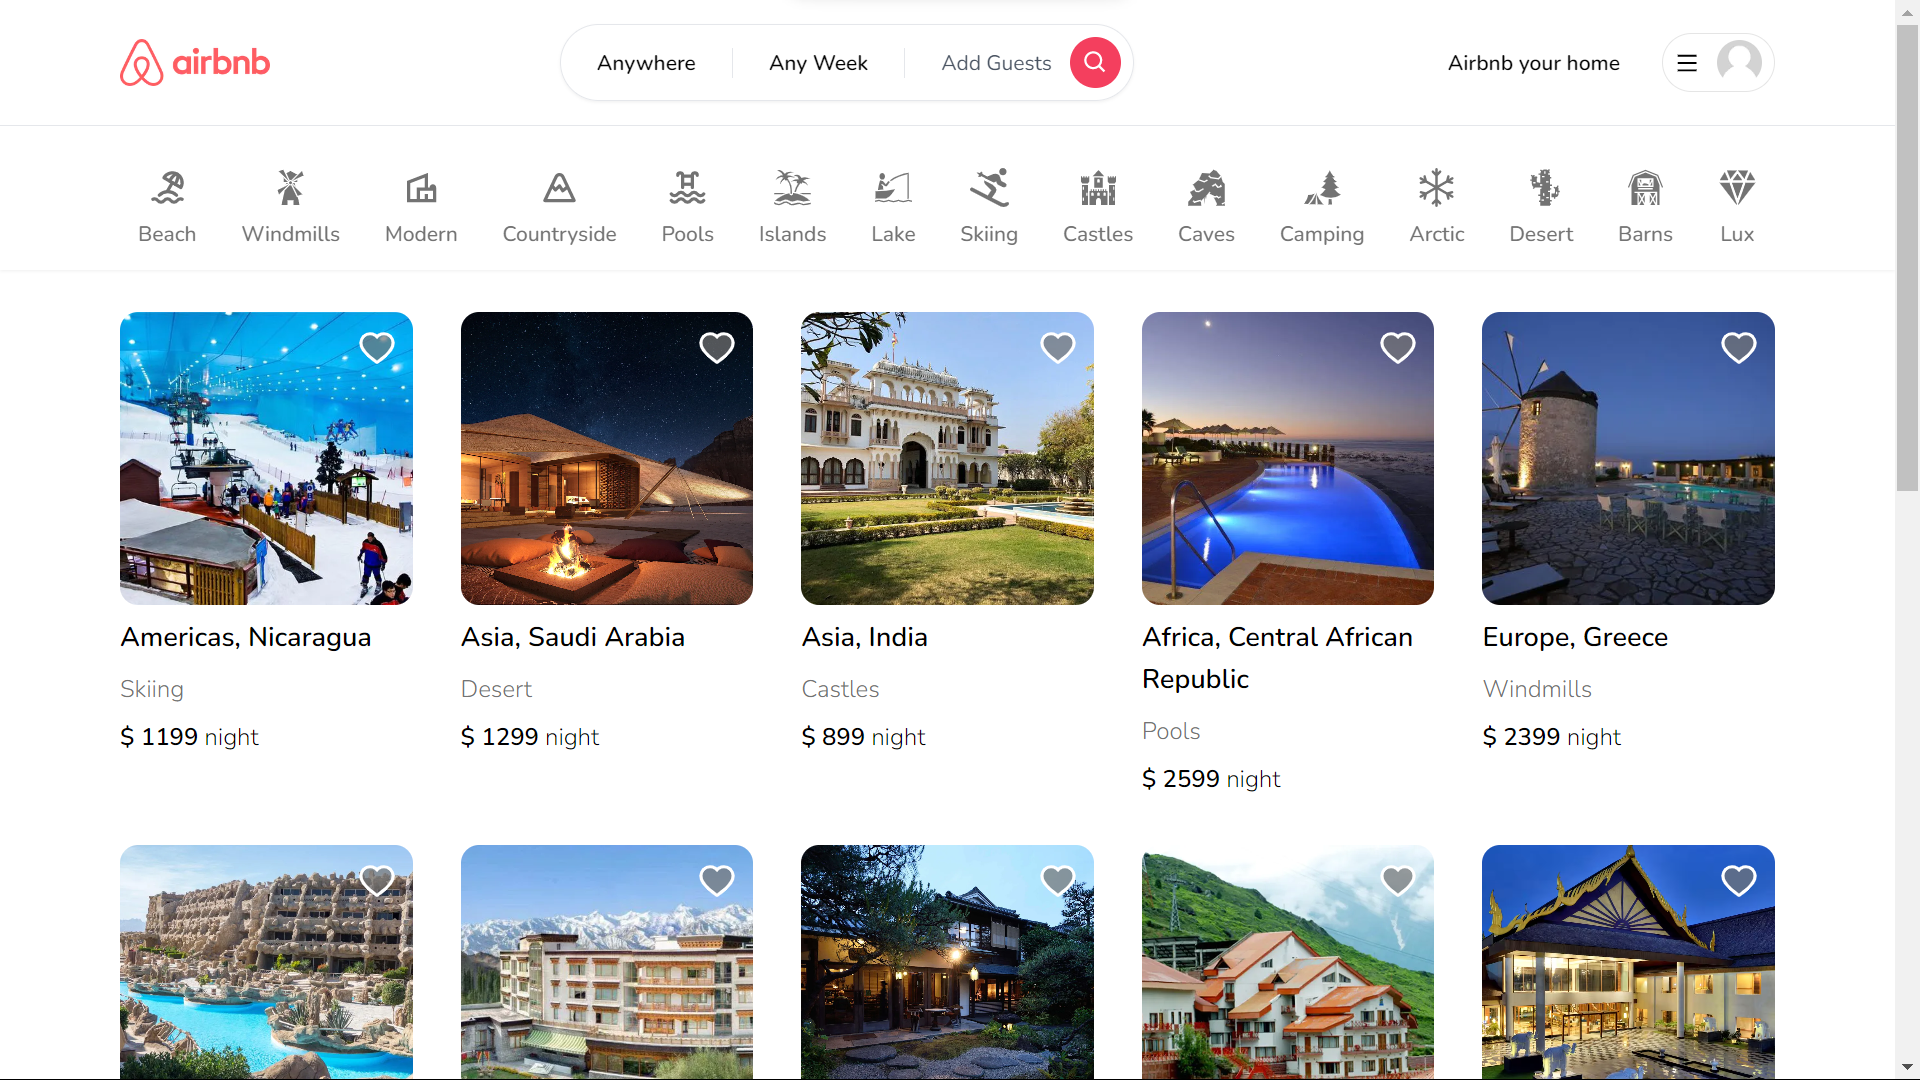
\includegraphics[scale=0.3]{chapters/images/home-page.png}
	\caption{Home page of the website}
\end{figure}

\begin{figure}[!h]
	\centering
	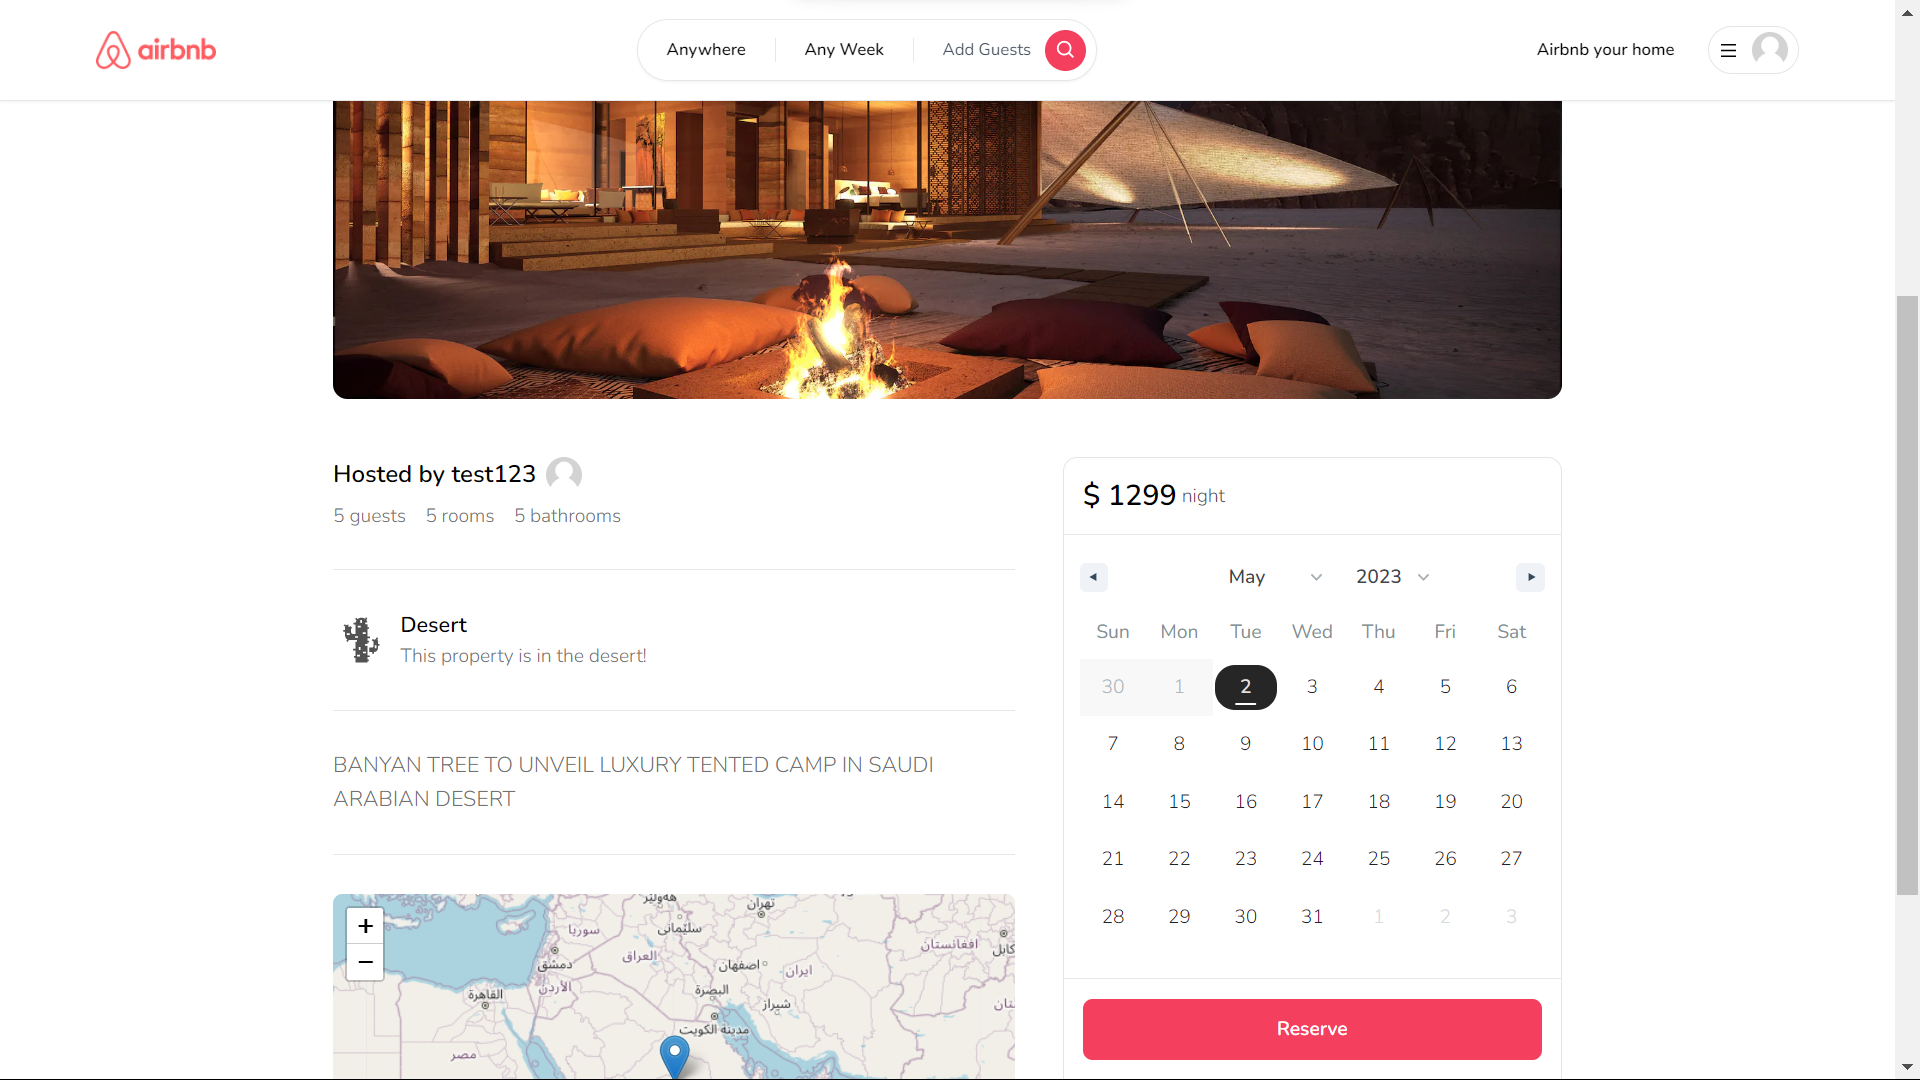
\includegraphics[scale=0.3]{chapters/images/listing-page.png}
	\caption{Page displaying information about a single listing}
\end{figure}

\begin{figure}[!h]
	\centering
	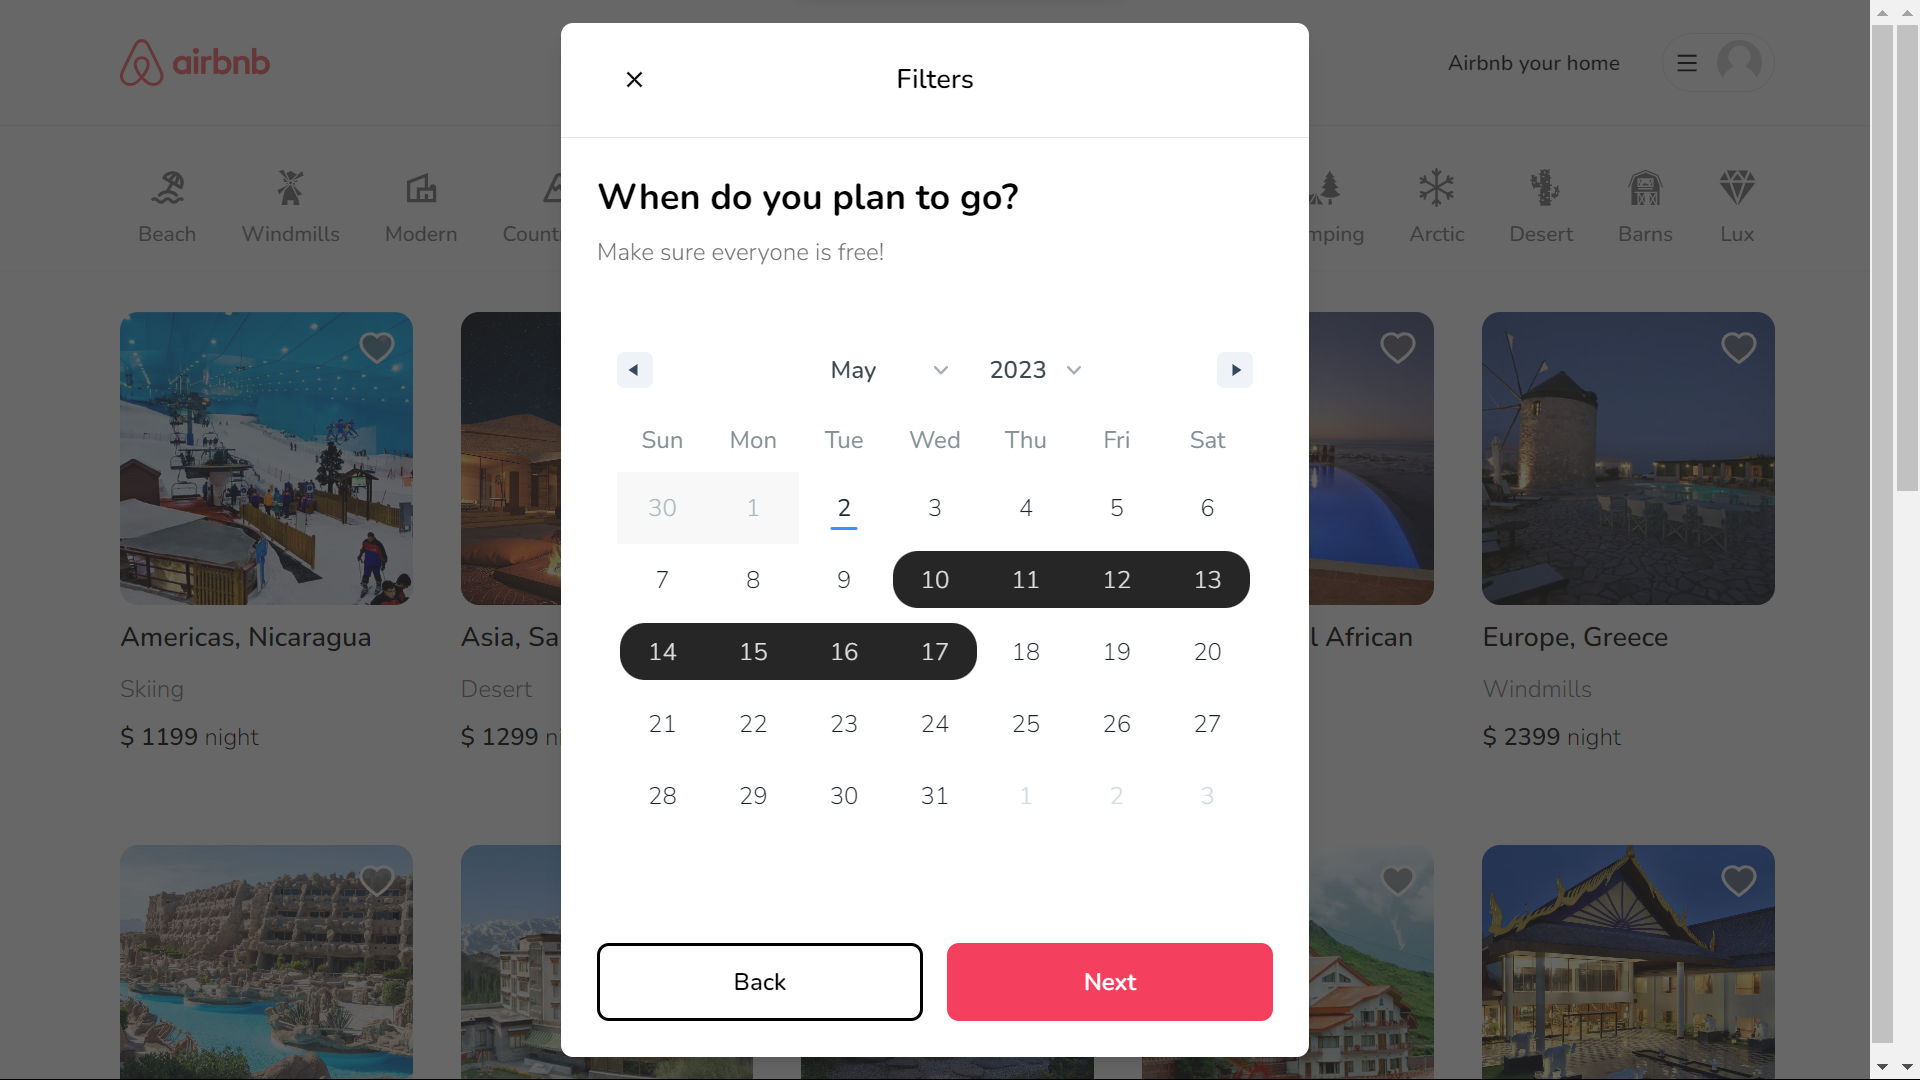
\includegraphics[scale=0.3]{chapters/images/filters-modal.png}
	\caption{Modal to apply filters on properties list}
\end{figure}

\begin{figure}[!h]
	\centering
	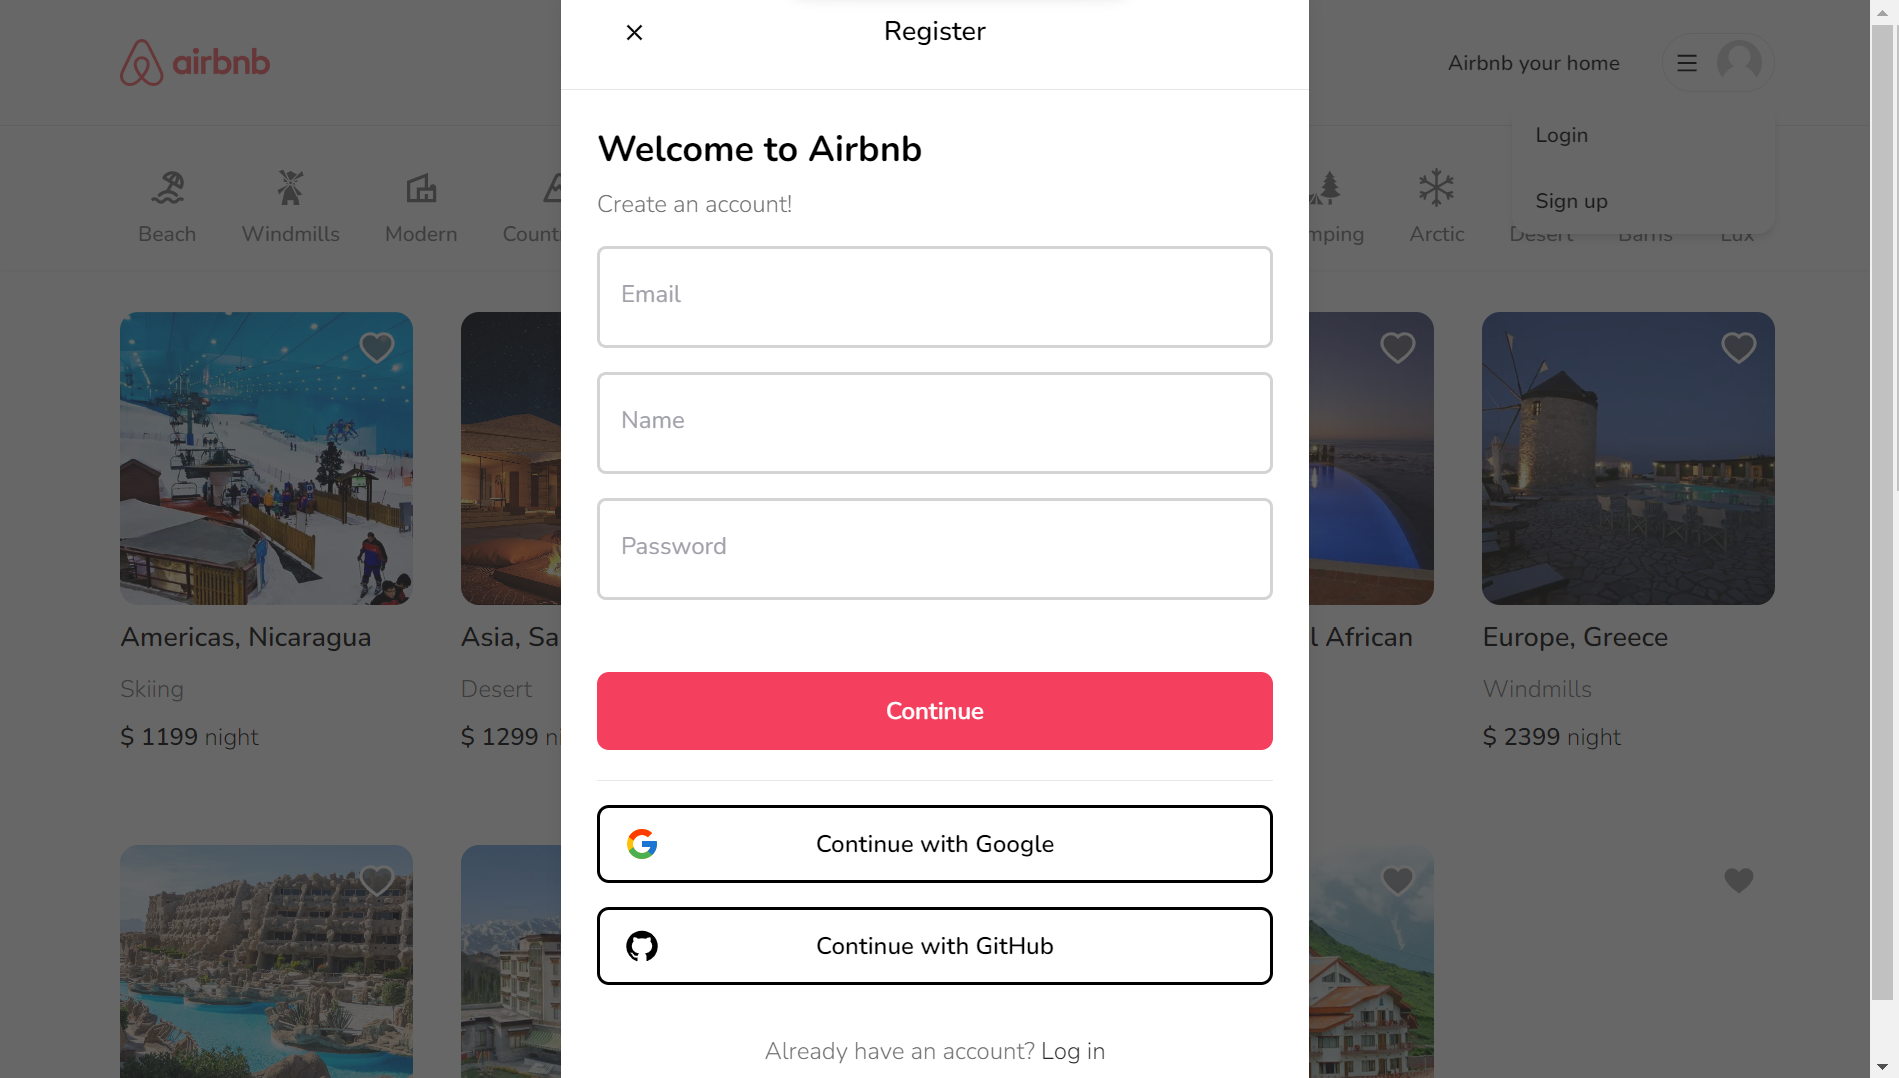
\includegraphics[scale=0.3]{chapters/images/registration-modal.png}
	\caption{Modal to register as a new user}
\end{figure}

\begin{figure}[!h]
	\centering
	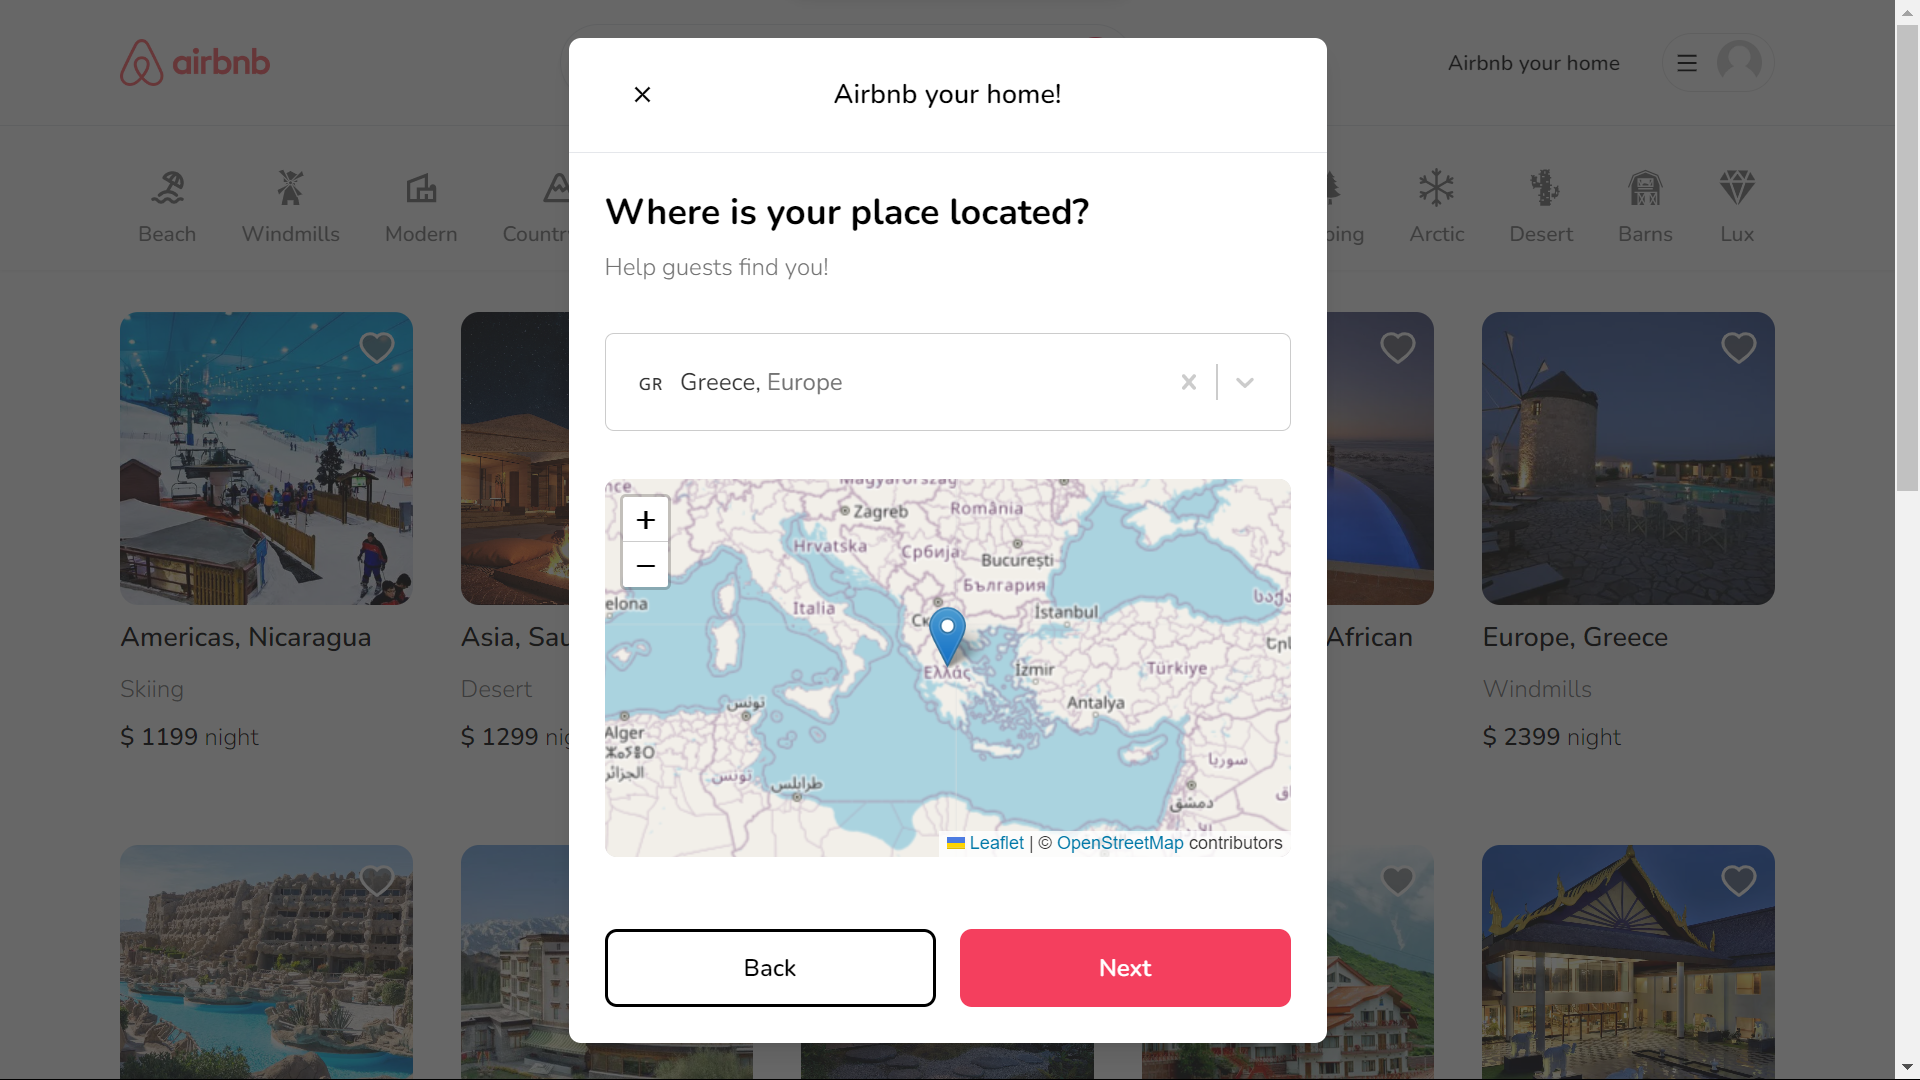
\includegraphics[scale=0.3]{chapters/images/listing-creation.png}
	\caption{Listing creation flow}
\end{figure}

\begin{figure}[!h]
	\centering
	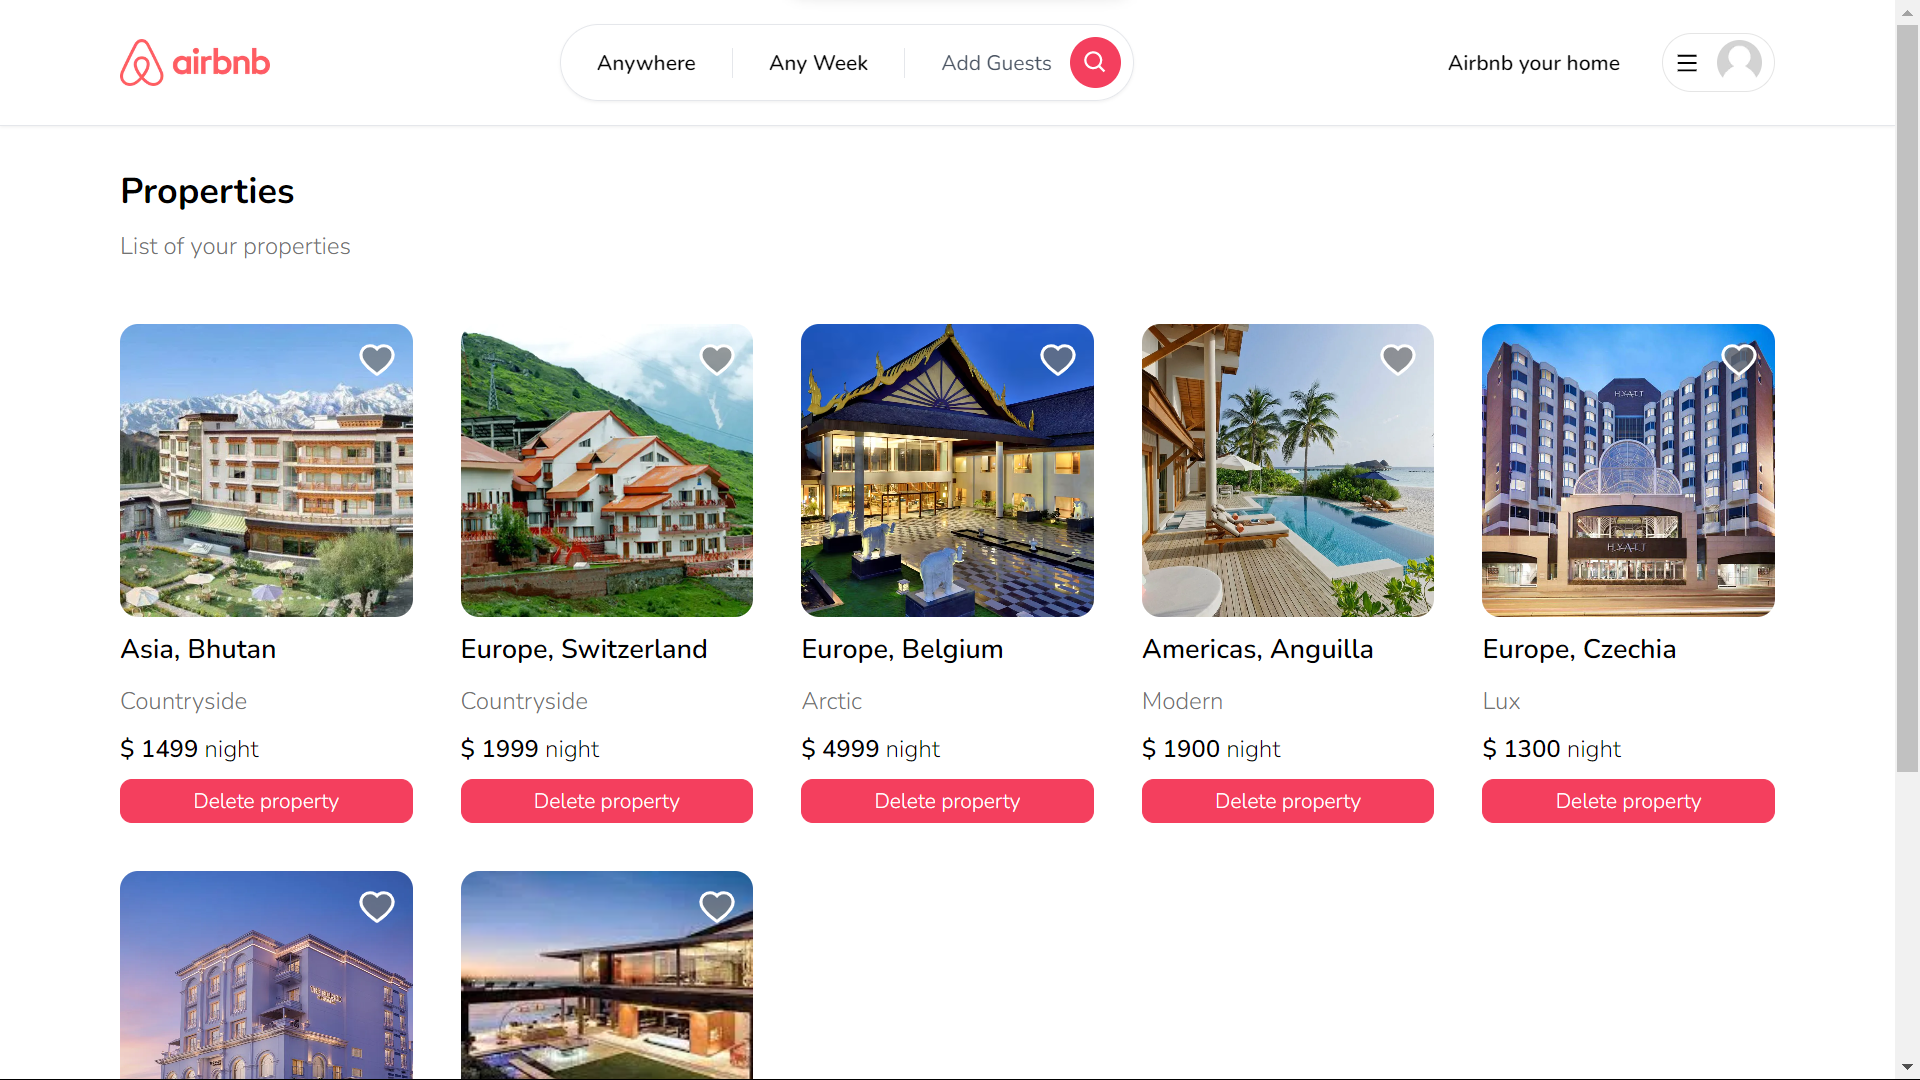
\includegraphics[scale=0.3]{chapters/images/properties-page.png}
	\caption{Property management page}
\end{figure}

\begin{figure}[!h]
	\centering
	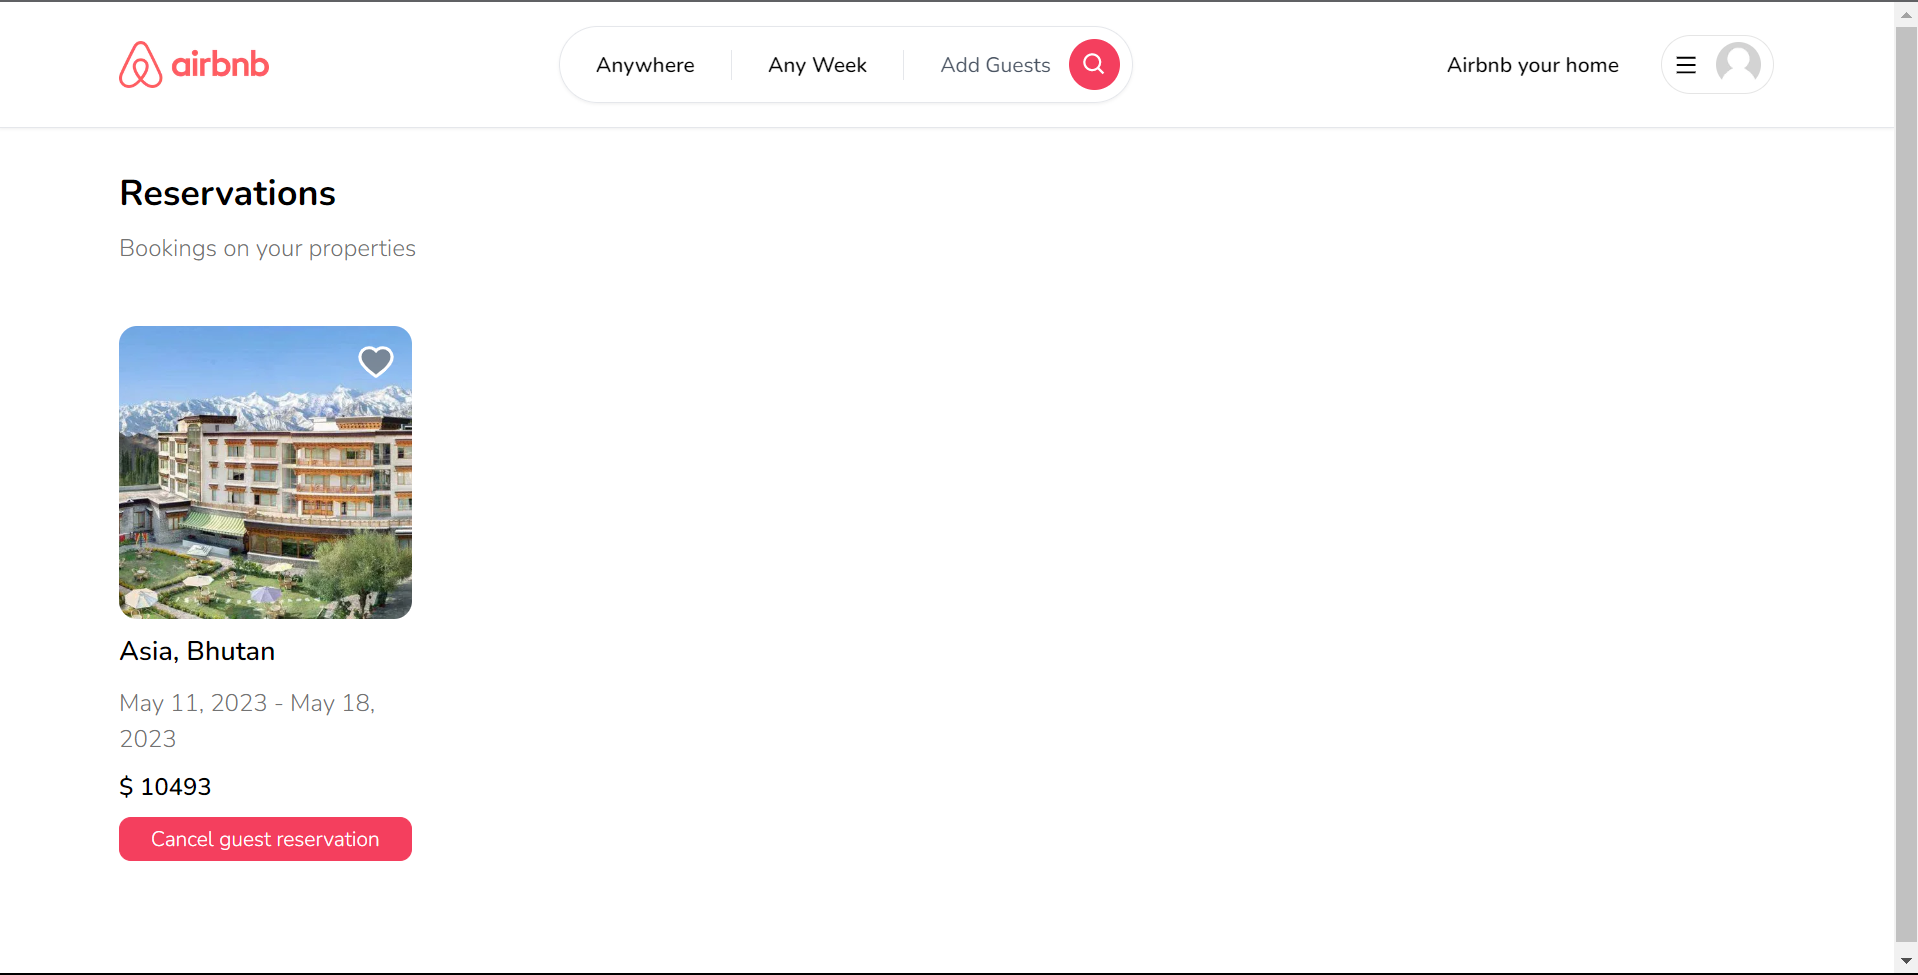
\includegraphics[scale=0.3]{chapters/images/reservation-management.png}
	\caption{Reservations management page}
\end{figure}

\section{Quality Assurance}
Although there was no dedicated QA team involved, quality assurance measures were taken during the implementation phase. These measures included the integration of ESLint into the codebase. ESLint was used to enforce coding standards, maintain code consistency, and identify potential errors or stylistic issues. By configuring ESLint with appropriate rules and plugins, the codebase was thoroughly checked for readability, maintainability, and correctness.

The implementation phase encompassed a structured approach, manual testing for functionality and user experience, visual representation through screenshots, and the integration of ESLint for maintaining code quality and consistency. These steps contributed to the successful development of the full stack application, resulting in a functional and user-friendly solution.

The deployed full stack application can be accessed at:\\ \href{https://rent-application-example.vercel.app/}{\underline{rent-application-example.vercel.app}}